%% Master's Thesis — Nidanur Günay
%% Abstraction Mechanisms for Virtual Avatars
%% University of Konstanz — Visual Computing
%% ============================================

\documentclass[
  11pt,
  a4paper,
  twoside,
  openany,
  headings=optiontohead,
  parskip=half,
]{scrbook}

%% ---- Encoding & Language ----
\usepackage[T1]{fontenc}
\usepackage[utf8]{inputenc}
\usepackage[english]{babel}
\usepackage{csquotes}

%% ---- Typography ----
% Body: Palatino serif (mathpazo); headings: Helvetica (\sffamily via helvet)
\usepackage{mathpazo}                % Palatino for body + math
\usepackage[scaled=0.90]{helvet}     % Helvetica for \sffamily headings
\usepackage{setspace}
\setstretch{1.15}
\usepackage{microtype}

%% ---- Paragraph style handled by parskip=half in \documentclass ----
\raggedbottom   % prevent vertical stretch on short pages (avoids big inter-paragraph gaps)

%% ---- Page Layout ----
\usepackage[
  a4paper,
  inner=3cm,
  outer=2.5cm,
  top=2.5cm,
  bottom=2.5cm,
  bindingoffset=5mm,
]{geometry}

%% ---- KOMA heading fonts (sans-serif, matching Fink thesis) ----
\setkomafont{chapter}{\normalfont\huge\sffamily}
\setkomafont{section}{\normalfont\large\sffamily}
\setkomafont{subsection}{\normalfont\normalsize\sffamily}
\setkomafont{subsubsection}{\normalfont\normalsize\sffamily\itshape}
\setkomafont{pagehead}{\normalfont\small\sffamily}
\setkomafont{pagenumber}{\normalfont\small\sffamily}

%% ---- Heading spacing (tighter, matching Fink thesis) ----
% Reduce the large default drop above/below chapter titles
\renewcommand*{\chapterheadstartvskip}{\vspace*{20pt}}
\renewcommand*{\chapterheadendvskip}{\vspace{8pt}}
% Tighten space before/after section-level headings
\RedeclareSectionCommand[beforeskip=0.75\baselineskip, afterskip=0.4\baselineskip]{section}
\RedeclareSectionCommand[beforeskip=0.6\baselineskip,  afterskip=0.4\baselineskip]{subsection}
\RedeclareSectionCommand[beforeskip=0.5\baselineskip,  afterskip=0.25\baselineskip]{subsubsection}

%% ---- Header / Footer ----
\usepackage[automark, headsepline]{scrlayer-scrpage}
\clearpairofpagestyles
\ohead{\headmark}
\ofoot[\pagemark]{\pagemark}

%% ---- Math ----
\usepackage{amsmath, amssymb, amsthm}
\usepackage{mathtools}

%% ---- Graphics & Figures ----
\usepackage{graphicx}
\graphicspath{{figures/}}
\usepackage{float}
\usepackage{subcaption}
\captionsetup{labelfont=bf, font=small, labelsep=colon, format=hang}
\usepackage{wrapfig}
\usepackage{tikz}
\usepackage{pgfplots}
\pgfplotsset{compat=1.18}

%% ---- Tables ----
\usepackage{booktabs}
\usepackage{tabularx}
\usepackage{multirow}
\usepackage{array}

%% ---- Algorithms & Code ----
\usepackage{algorithm}
\usepackage{algpseudocode}
\usepackage{listings}
\usepackage{xcolor}

\definecolor{codegray}{rgb}{0.5,0.5,0.5}
\definecolor{codeblue}{rgb}{0.13,0.29,0.53}
\definecolor{codegreen}{rgb}{0.0,0.5,0.0}
\definecolor{codepurple}{rgb}{0.58,0,0.82}
\definecolor{backcolour}{rgb}{0.97,0.97,0.97}

\lstdefinestyle{mystyle}{
  backgroundcolor=\color{backcolour},
  commentstyle=\color{codegreen},
  keywordstyle=\color{codeblue}\bfseries,
  numberstyle=\tiny\color{codegray},
  stringstyle=\color{codepurple},
  basicstyle=\ttfamily\small,
  breakatwhitespace=false,
  breaklines=true,
  captionpos=b,
  keepspaces=true,
  numbers=left,
  numbersep=5pt,
  showspaces=false,
  showstringspaces=false,
  showtabs=false,
  tabsize=2,
  frame=single,
  rulecolor=\color{gray!30},
}
\lstset{style=mystyle}

%% ---- Hyperlinks & PDF Metadata ----
\usepackage[
  pdftitle={Abstraction Mechanisms for Virtual Avatars},
  pdfauthor={Nidanur Günay},
  pdfsubject={Master's Thesis, University of Konstanz},
  pdfkeywords={non-photorealistic rendering, VR avatars, abstraction, trust, Meta Avatar SDK},
  colorlinks=true,
  linkcolor=black,
  citecolor=black,
  urlcolor=blue,
  bookmarks=true,
  bookmarksopen=true,
]{hyperref}
\usepackage{bookmark}

%% ---- Bibliography ----
\usepackage[
  backend=biber,
  style=ieee,
  sorting=none,
  maxbibnames=10,
]{biblatex}
\addbibresource{references.bib}

%% ---- Acronyms & Glossary ----
\usepackage[acronym, toc, nonumberlist]{glossaries}
\makeglossaries
%% Acronyms — add entries as needed
%% Usage in text: \gls{gpu}, \acrfull{cnn}

\newacronym{gpu}{GPU}{Graphics Processing Unit}
\newacronym{cpu}{CPU}{Central Processing Unit}
\newacronym{cnn}{CNN}{Convolutional Neural Network}
\newacronym{ml}{ML}{Machine Learning}
\newacronym{dl}{DL}{Deep Learning}
\newacronym{api}{API}{Application Programming Interface}
\newacronym{rgb}{RGB}{Red Green Blue}
\newacronym{hdr}{HDR}{High Dynamic Range}
\newacronym{fps}{FPS}{Frames Per Second}
\newacronym{vr}{VR}{Virtual Reality}
\newacronym{ar}{AR}{Augmented Reality}


%% ---- Theorem Environments ----
\theoremstyle{plain}
\newtheorem{theorem}{Theorem}[chapter]
\newtheorem{lemma}[theorem]{Lemma}
\newtheorem{proposition}[theorem]{Proposition}
\newtheorem{corollary}[theorem]{Corollary}

\theoremstyle{definition}
\newtheorem{definition}[theorem]{Definition}
\newtheorem{example}[theorem]{Example}

\theoremstyle{remark}
\newtheorem{remark}[theorem]{Remark}

%% ---- Utilities ----
\usepackage{lipsum}   % placeholder text — remove when writing
\usepackage{todonotes}
\usepackage{cleveref}

%% ========================================================
\begin{document}

%% ---- Front Matter ----
\KOMAoptions{open=any}
\frontmatter
%% Title Page — University of Konstanz
\begin{titlepage}
  \sffamily
  \begin{center}

    \vspace*{2.5cm}
    {\huge Abstraction Mechanisms\\[0.25em] for Virtual Avatars}\\[3em]

    {\large Master's Thesis}\\[2.5em]

    submitted by\\[0.6em]
    {\large Nidanur Günay}\\[3em]

    at the\\[2em]

    
\includegraphics[width=0.42\textwidth]{UniKonstanz_Logo_Minimum_sRGB}\\[2.5em]

    Department of Computer and Information Science\\[2.5em]

    \begin{tabular}{r@{\hspace{1.5em}}l}
      1. Reviewer: & Prof.\ Dr.\ Oliver Deussen \\[0.5em]
      2. Reviewer: & Prof.\ Dr.\ Tiare Feuchtner \\
    \end{tabular}\\[4em]

    Konstanz, 2026

  \end{center}
\end{titlepage}
\newpage

%% Abstract
\chapter*{Abstract}
\addcontentsline{toc}{chapter}{Abstract}

Virtual reality applications increasingly rely on avatar representations to facilitate social presence and user embodiment. However, photorealistic avatar rendering can trigger the uncanny valley effect, where near-realistic human representations evoke discomfort and reduced trust rather than engagement. Non-photorealistic rendering~(NPR) offers a principled alternative, deliberately abstracting avatar appearance while preserving expressiveness and identity.

This thesis presents the design, implementation, and evaluation of a real-time NPR stylisation system for virtual avatars. Eight techniques were developed iteratively: geometry-based inverted hull outlines, screen-space normal edge detection, Sobel edge detection with adaptive skin-to-clothing thresholding, Gaussian pre-filtered Sobel, hierarchical multi-cue edge detection combining depth, normal, and colour discontinuities, isotropic Kuwahara painterly filtering, and two composite techniques combining painterly abstraction with edge rendering. The techniques were implemented and compared across three avatar platforms — a Mixamo humanoid model, the Meta Avatars SDK, and Avaturn — to assess their visual behaviour and robustness under different mesh topologies and rendering pipelines. Avaturn was selected as the primary platform for the user study due to its facial rigging capabilities and higher photorealistic fidelity.

The user study investigates how visual abstraction affects the perceived trustworthiness of an avatar delivering advice. Participants watched short video scenarios in which a speaker — presented either as a real person, a photorealistic Avaturn avatar, or an NPR-stylised avatar — recommended one of two options in a practical decision situation. After each scenario, participants rated how trustworthy they found the speaker's recommendation. The results provide empirical insight into the relationship between avatar abstraction level and social trust, offering practical guidance for avatar design in applications where perceived credibility matters.

\bigskip
\noindent\textbf{Keywords:} non-photorealistic rendering, virtual reality, avatar abstraction, trust perception, edge detection, Avaturn, uncanny valley, Kuwahara filter.

\newpage

%% Acknowledgements
\chapter*{Acknowledgements}
\addcontentsline{toc}{chapter}{Acknowledgements}

I would like to express my sincere gratitude to my supervisor, Prof.\ Dr.\ Oliver Deussen, for his guidance, continuous support, and invaluable feedback throughout this thesis. His expertise in computer graphics and visual computing shaped the direction of this work in meaningful ways.

I am also deeply grateful to my co-supervisor, Prof.\ Dr.\ Tiare Feuchtner, for her insightful discussions, encouragement, and thoughtful advice — particularly on the human factors and user study aspects of this research. Her perspective was essential in connecting the technical work to its broader perceptual context.

Special thanks go to my colleagues at the Visual Computing Group at the University of Konstanz for the stimulating academic environment and helpful conversations throughout this journey.

Finally, I am grateful to my family and friends for their patience, understanding, and unwavering support.

\newpage


\tableofcontents
\listoffigures
\listoftables
%% Abbreviations
\chapter*{Abbreviations}
\addcontentsline{toc}{chapter}{Abbreviations}

\begin{tabular}{@{}lp{0.75\textwidth}@{}}
  ANOVA  & Analysis of Variance \\[0.3em]
  API    & Application Programming Interface \\[0.3em]
  AR     & Augmented Reality \\[0.3em]
  CG     & Computer-Generated \\[0.3em]
  ESF    & Extensible Shader Framework \\[0.3em]
  FPS    & Frames Per Second \\[0.3em]
  GPU    & Graphics Processing Unit \\[0.3em]
  HCI    & Human-Computer Interaction \\[0.3em]
  HLSL   & High-Level Shading Language \\[0.3em]
  HMD    & Head-Mounted Display \\[0.3em]
  HSV    & Hue, Saturation, Value (colour space) \\[0.3em]
  LOD    & Level of Detail \\[0.3em]
  NPR    & Non-Photorealistic Rendering \\[0.3em]
  PBR    & Physically-Based Rendering \\[0.3em]
  RGB    & Red, Green, Blue \\[0.3em]
  SDK    & Software Development Kit \\[0.3em]
  SSS    & Subsurface Scattering \\[0.3em]
  UI     & User Interface \\[0.3em]
  URP    & Universal Render Pipeline \\[0.3em]
  UV     & Texture Coordinate Axes (U and V) \\[0.3em]
  VR     & Virtual Reality \\
\end{tabular}

\newpage

\KOMAoptions{open=any}

%% ---- Main Matter ----
\mainmatter
%% Chapter 1 — Introduction
\chapter{Introduction}
\label{ch:introduction}

\section{Motivation}
\label{sec:motivation}

Communication through avatars has become a defining feature of virtual reality, extending well beyond its origins as a navigational convenience to serve as the primary medium through which users express identity, signal intent, and form social relationships in shared digital environments.
The perceptual consequences of this shift are well documented.
Avatar appearance exerts a measurable influence on social presence and interpersonal trust, meaning that the visual design of an avatar functions as a communicative act in its own right, shaping how users are perceived and how they engage with one another~\cite{nowak2003, weidner2023}.

Recent advances in generative AI have made photorealistic avatar creation more accessible than ever.
Platforms such as Avaturn can now produce a fully rigged, expressively animated CG avatar from a single uploaded photograph, reconstructing facial geometry and surface appearance with a degree of fidelity that was difficult to achieve outside of dedicated production pipelines only a few years ago.
The implicit promise of this technology is that a digital representation close enough to the real person will be received as one.
Yet this is precisely where a well-known perceptual problem arises.
Mori's uncanny valley hypothesis, first proposed in 1970, predicts that as a human representation approaches but falls just short of true photorealistic fidelity, it tends to evoke unease rather than familiarity~\cite{mori1970}.
An avatar that comes close to realism without quite reaching it can therefore undermine the very trust it was designed to support, a finding corroborated across robotics, computer graphics, and virtual environment research.

Non-photorealistic rendering~(NPR) offers a different path through this problem.
Rather than simulating accurate lighting and surface detail, NPR techniques deliberately stylise the rendered output to achieve artistic or communicative goals~\cite{gooch1998}.
Cel shading, edge line drawing, and painterly filtering can each abstract an avatar's appearance in ways that sidestep the uncanny valley, while preserving enough expressiveness and readable identity that the character remains engaging.
The open question is not whether this looks appealing.
It is whether a deliberately abstracted avatar can still be trusted by the people interacting with it, or whether reducing realism introduces its own perceptual costs.
That question has received surprisingly little attention in the context of modern, SDK-managed avatar systems.

\section{Problem Statement}
\label{sec:problem_statement}

Applying NPR stylisation to photorealistic avatar systems is not straightforward.
Production avatar platforms each manage rendering through their own shader architectures, material systems, and mesh topologies, and integrating custom visual effects into these pipelines without disrupting avatar fidelity or performance requires working within constraints that most prior NPR research has not had to address.
Existing work on NPR for virtual characters largely operates on custom assets built under full authorial control.
How NPR techniques behave when applied across platforms with different rendering architectures, and which constraints prove most limiting in practice, is not well established.

Beyond this technical question, there is an open empirical one.
Photorealistic avatar generation has become increasingly accessible, yet the uncanny valley problem suggests that realism alone does not guarantee a positive reception.
Whether NPR abstraction can improve how an avatar is perceived, specifically in terms of trustworthiness, and how much stylisation is too much before credibility is lost, are questions that remain largely unanswered.
They matter for any application where avatar credibility is at stake: social VR, remote consultation, education, and more.

This thesis addresses both challenges.
It examines how NPR techniques can be applied across avatar platforms with differing rendering constraints, and asks whether the resulting visual abstraction affects the trust that viewers place in an avatar delivering a recommendation.

\section{Contributions}
\label{sec:contributions}

This thesis makes the following contributions:

\begin{itemize}
  \item \textbf{Multi-platform NPR shader system.}
    A real-time NPR stylisation system is developed and applied across three avatar platforms: a Mixamo humanoid model used for initial technique development, the Meta Avatars SDK integrated via the app-specific post-lighting fragment hook~(\texttt{AppSpecificPostManipulation}), and Avaturn, which serves as the primary platform for the user study.
    The cross-platform implementation reveals the constraints and trade-offs specific to each rendering pipeline and demonstrates that the core NPR techniques generalise across different mesh topologies and material systems.

  \item \textbf{Iteratively developed stylisation techniques.}
    A series of techniques are designed, implemented, and compared through an iterative development process:
    toon shading with a quantized diffuse model,
    X-Toon extended toon shading with a depth-indexed 2D ramp,
    screen-space normal edge detection,
    Sobel edge detection with adaptive skin-to-clothing thresholding,
    Gaussian pre-filtered Sobel,
    hierarchical multi-cue edge detection combining depth, normal, and colour discontinuities,
    isotropic Kuwahara painterly filtering,
    Kuwahara combined with Sobel edge lines,
    and a composite technique combining Kuwahara, Gaussian Sobel, and hierarchical detection.
    Each technique addresses limitations observed in its predecessor, and all are selectable at runtime without recompilation.
    A final technique is selected for the user study based on visual assessment across all three avatar platforms.

  \item \textbf{In-VR parameter tuning interface.}
    A fully procedural, WorldSpace UI panel is implemented in Unity, enabling live exploration of all shader parameters from inside the headset using controller raycasting.
    This tool was central to the iterative development process and can be reused for future shader experimentation.

  \item \textbf{Video-based user study on avatar abstraction and trust.}
    A user study is conducted using pre-recorded video scenarios in which a speaker, shown as either a real person, a photorealistic Avaturn avatar, or an NPR-stylised avatar, recommends one of two options in a practical decision situation.
    The video format is chosen deliberately: it is the only medium that allows a real human speaker and avatar counterparts to be compared under identical viewing conditions.
    The study provides empirical insight into how visual abstraction affects the perceived trustworthiness of an avatar's advice.
\end{itemize}

\section{Thesis Outline}
\label{sec:outline}

The remainder of this thesis is structured as follows:

\begin{description}
  \item[\Cref{ch:related_work}] surveys prior work on NPR for 3D characters, avatar rendering and realism in VR, and trust and perception in virtual environments, positioning this thesis in the existing research landscape.

  \item[\Cref{ch:background}] introduces the technical and theoretical foundations required for this work, covering edge detection mathematics, the Kuwahara filter, the Meta Avatars SDK rendering pipeline, and concepts of trust and abstraction from human-computer interaction.

  \item[\Cref{ch:methodology}] presents the research questions, the overall system design, the iterative development strategy, and the user study design.

  \item[\Cref{ch:implementation}] describes the full implementation of the NPR shader system, covering all eight techniques in detail, the runtime tooling, and the rationale for the final technique selection used in the user study.

  \item[\Cref{ch:evaluation}] reports the technical evaluation of each stylisation technique and presents the results of the user study, followed by a discussion of the findings and their implications.

  \item[\Cref{ch:conclusion}] summarises the contributions of this thesis, reflects on its limitations, and outlines directions for future work.
\end{description}

%% Chapter 2 — Related Work
\chapter{Related Work}
\label{ch:related_work}

\section{Non-Photorealistic Rendering for 3D Characters}
\label{sec:related_npr}

Non-photorealistic rendering has a substantial history in computer graphics, though most of it predates the era of closed, SDK-managed avatar systems. Understanding this body of work requires distinguishing between the underlying techniques — edge detection, shading stylisation, and painterly filtering — and their specific application to animated human figures.

The foundational contribution to NPR lighting is the cool-to-warm shading model introduced by Gooch et al.~\cite{gooch1998}, which replaced the continuous Lambertian diffuse term with a hue shift from cool shadows to warm highlights, mimicking the conventions of technical illustration. While the model targets engineering drawings rather than characters, its core insight — that shading can communicate form without physically simulating light — became a reference point for subsequent stylised rendering work. In the context of this thesis, the more direct technical heritage lies in outline extraction and edge-based effects rather than shading models.

Silhouette rendering has been approached from two geometrically distinct directions. Geometry-based methods generate outlines using the GPU rasteriser itself. The inverted hull technique, described by Lake et al.~\cite{lake2000}, expands back-facing polygons along vertex normals by a small offset, creating a slightly enlarged shell of the mesh. When the front-facing geometry is rendered on top, only the protruding rim remains visible as an outline. The approach requires no image-space computation, scales predictably with polygon count, and remains consistent regardless of camera distance — properties that make it well suited to animated characters in real-time applications. Isenberg et al.~\cite{isenberg2003} provide a systematic survey of silhouette algorithms and conclude that geometry-based methods are robust and distance-independent, but structurally incapable of detecting internal surface detail. This limitation matters for avatar rendering, where facial features, clothing folds, and skin creases all constitute expressive visual cues that lie within the silhouette boundary.

Image-space methods operate on the rasterised output rather than on the mesh directly. Screen-space normal derivatives, computed via the hardware-accelerated \texttt{ddx}/\texttt{ddy} intrinsics available on all modern GPUs, detect abrupt changes in surface orientation without any additional draw calls or intermediate render targets. This approach captures surface creases and mesh boundaries that geometry expansion misses. The fundamental limitation is that edge thickness is measured in screen pixels rather than world-space units, so edges scale with camera distance. In an immersive VR context where the user moves relative to other participants, this produces edges that appear overly thick at close range and invisible at distance.

Texture-based edge detection targets a different layer of information. The Sobel operator~\cite{gonzalez2018}, a discrete gradient approximation applied to the diffuse texture via a $3\times3$ convolution kernel, identifies luminance boundaries that correspond to clothing patterns, facial contours, and painted surface details. Unlike geometry-based methods, it responds to what was painted onto the surface rather than to the surface shape itself. The approach is well established in image processing~\cite{canny1986}, but differentiation inherently amplifies high-frequency noise. Marr and Hildreth~\cite{marr1980} demonstrated that low-pass pre-filtering is a prerequisite for stable gradient computation, an observation that motivates the Gaussian pre-filtered variant explored later in this work.

Extended toon shading approaches have explored richer parameter spaces. Barla et al.~\cite{barla2006} introduced X-Toon, which parameterises the shading tone ramp by both view angle and depth, enabling a two-dimensional lookup that encodes artistic intent unavailable in a one-dimensional quantisation step. On the painterly side, the Kuwahara filter — originally a noise-reduction tool in medical imaging — has been applied to NPR as a means of producing region-based painterly abstraction without explicit edge detection. Kyprianidis et al.~\cite{kyprianidis2009} extended the isotropic variant with an anisotropic formulation aligned to local image structure, producing brush-stroke effects oriented along salient contours. The anisotropic extension requires a structure tensor computed from a prior render pass and cannot be implemented within a single-pass fragment hook — a constraint directly relevant to the integration target in this thesis.

Hatching represents a separate branch of character NPR in which tonal regions are conveyed by oriented stroke textures rather than flat fills or edge lines~\cite{praun2001}. While visually distinctive, the approach depends heavily on stroke coherence across animation frames, a problem that has not been fully solved in real-time settings. It was not pursued in this work.

What connects nearly all of these contributions is an implicit assumption: the developer controls the rendering pipeline. Techniques are designed and evaluated against custom meshes, open rendering frameworks, or research engines where shader code, render passes, and material systems can be freely modified. This assumption does not hold for production avatar SDKs.

\section{Avatar Rendering and Appearance in VR}
\label{sec:related_vr_avatars}

Commercial avatar platforms have matured considerably beyond the research systems used in early social VR studies. The Meta Avatars SDK, used in Horizon Worlds and accessible to third-party developers, provides production-quality physically-based rendering with subsurface scattering for skin, procedural eye glints, hair rendering, and compute-based GPU skinning driven by body tracking data. The pipeline is generated and managed by Meta's Extensible Shader Framework~(ESF), which exposes a small number of application-specific fragment hooks while keeping the core lighting computations proprietary and unmodifiable. This architecture maintains pipeline integrity across SDK updates and ensures consistent quality across hardware, but it substantially constrains where custom rendering logic can be inserted.

Prior NPR work applied to avatar systems has generally assumed open pipeline access. Studies applying toon shading or stylisation to VR avatars have used custom character models with fully accessible shader code, or have modified appearance at the asset level before the render pipeline is involved. Applying NPR to a closed, compute-skinned, LOD-managed avatar at runtime — without SDK modification, without additional render passes, and without breaking the material management system — has not been addressed in the published literature to the author's knowledge.

The most directly related work on avatar stylisation and perception is Canales et al.~\cite{canales2024}, who conducted a controlled study of how avatar stylisation level affects perceived trust. Participants interacted with avatars at varying degrees of abstraction, from photorealistic to explicitly cartoon-like, and rated trustworthiness using social cognition instruments. The study found that moderate stylisation did not reduce trust relative to photorealistic rendering, and could in some conditions improve it, consistent with the uncanny valley framework. However, the stylisation was applied to custom assets in an open pipeline, and the technique variations compared were coarse-grained — the distinction between different edge detection approaches, painterly filtering methods, or composite techniques was not investigated. The work demonstrates that abstraction matters; it leaves open the question of which specific technical approach is most effective and whether these findings generalise to SDK-managed avatars.

Weidner and Broll~\cite{weidner2023} examined how avatar visual fidelity interacts with self-embodiment and social perception in video conferencing and VR contexts. Their findings indicate that the visual design of an avatar does not operate independently of the observer's sense of identification with it: fidelity effects on social judgements are mediated by embodiment. This has methodological implications for user studies that compare avatar conditions — a participant's prior exposure to and familiarity with a particular avatar style can influence their trust ratings independently of the stylisation itself.

\section{Trust, Social Presence, and the Uncanny Valley}
\label{sec:related_vr_trust}

The uncanny valley hypothesis, first articulated by Mori~\cite{mori1970}, proposes that human affinity for a human-like representation increases with resemblance up to a point, then drops sharply before recovering near perfect replication. The drop is attributed to a mismatch: a near-realistic representation triggers expectations calibrated for real humans, but subtle violations — in motion timing, skin texture, eye movement — produce unease rather than familiarity. MacDorman and Ishiguro~\cite{macdorman2006} provided empirical support for this in the context of humanoid robots, documenting the eeriness ratings that emerge when a representation is close but not convincingly human.

Modern avatar systems sit squarely in the region of this curve that is most problematic. They achieve surface realism sufficient to trigger high perceptual expectations, but cannot fully meet those expectations in motion timing, facial micro-expressions, or gaze behaviour. The practical consequence for social VR is that a photorealistic avatar may actively undermine the sense of trustworthiness that it was designed to support. NPR stylisation provides a principled alternative: by moving the representation away from near-photorealism and into a clearly artistic register — cel shading, ink-line treatment, painterly filtering — the avatar exits the uncanny valley zone rather than attempting to cross it.

The relationship between avatar appearance and social presence has been studied extensively. Nowak and Biocca~\cite{nowak2003} demonstrated that anthropomorphism and perceived agency are distinct constructs that contribute independently to social presence and copresence. Counterintuitively, very high levels of visual anthropomorphism did not consistently produce higher social presence scores. This suggests that the social and perceptual response to an avatar is not a simple monotonic function of visual realism, and that stylisation does not necessarily carry a social cost.

Trust in the context of virtual agents is related to social presence but distinct from it. A user can experience strong co-presence with an avatar while trusting the entity it represents very little, or trust a stylised character precisely because it does not trigger uncanny valley discomfort. The literature on avatar trust has largely compared coarse conditions — human versus clearly robotic, photorealistic versus cartoonish — without exploring the design space within NPR itself. Whether a Kuwahara-painterly avatar is trusted differently from a Sobel-edge-line avatar, or whether hierarchical multi-cue edge detection produces a better trust outcome than a simpler screen-space method, are questions that have not been addressed.

\section{Summary and Positioning}
\label{sec:related_positioning}

The technical NPR literature provides a rich set of established techniques, developed and validated in open rendering environments. The social VR literature demonstrates that avatar appearance significantly affects trust and social presence, and that the uncanny valley poses a genuine design challenge for photorealistic avatar systems. Canales et al. showed that stylisation can improve trust outcomes; Nowak and Biocca established that the appearance–presence relationship is non-linear. What is missing is the intersection: a systematic investigation of fine-grained NPR technique choice on a production, SDK-managed avatar system, paired with an empirical measure of the trust response those choices produce.

This thesis addresses that gap. It integrates a suite of NPR techniques into the Meta Avatars SDK under real production constraints, evaluates the visual and performance trade-offs across techniques, and measures the trust implications of different abstraction levels in a user study.

%% Chapter 3 — Background
\chapter{Background}
\label{ch:background}

This chapter introduces the technical and theoretical foundations required for the work described in subsequent chapters. It covers the concept of virtual avatars and visual representation, edge detection mathematics, the Kuwahara painterly filter, and the human factors concepts of trust and social presence relevant to the user study.

\section{Mathematical Notation}
\label{sec:notation}

Throughout this thesis, scalars are denoted by italic letters~$x$, vectors by bold lowercase letters~$\mathbf{x}$, and matrices by bold uppercase letters~$\mathbf{X}$. The $i$-th element of vector $\mathbf{x}$ is written $x_i$. Convolution of a signal $I$ with a kernel $K$ is written $K * I$. In shader pseudocode, \texttt{ddx(f)} and \texttt{ddy(f)} refer to the hardware-computed screen-space partial derivatives of a value~\texttt{f} with respect to the horizontal and vertical screen axes, respectively.

\section{Edge Detection}
\label{sec:background_edge}

An edge in an image is conventionally defined as a location where intensity changes rapidly. Detecting such locations involves estimating the spatial gradient of the image intensity function, then applying a threshold to identify pixels where the gradient magnitude exceeds some criterion.

\subsection{Gradient-Based Detection}
\label{sec:background_gradient}

Given an image $I(x, y)$, the gradient is the vector $\nabla I = (\partial I / \partial x, \, \partial I / \partial y)$. Its magnitude
\begin{equation}
  M = \|\nabla I\| = \sqrt{\left(\frac{\partial I}{\partial x}\right)^2 + \left(\frac{\partial I}{\partial y}\right)^2}
  \label{eq:gradient_magnitude}
\end{equation}
provides a scalar measure of edge strength at each pixel. In practice, the partial derivatives are approximated by discrete convolution with finite-difference kernels.

The Sobel operator~\cite{gonzalez2018} estimates the gradient using two $3\times3$ kernels:
\begin{equation}
  G_x = \begin{bmatrix} -1 & 0 & +1 \\ -2 & 0 & +2 \\ -1 & 0 & +1 \end{bmatrix}, \qquad
  G_y = \begin{bmatrix} +1 & +2 & +1 \\ 0 & 0 & 0 \\ -1 & -2 & -1 \end{bmatrix}.
  \label{eq:sobel_kernels}
\end{equation}
$G_x$ responds to horizontal intensity transitions (vertical edges); $G_y$ responds to vertical transitions. The gradient magnitude is $M = \sqrt{G_x^2 + G_y^2}$, computed pointwise after convolving the image with each kernel separately. The $\pm2$ weights along the central row and column give the Sobel operator a small amount of spatial smoothing relative to the simpler Prewitt kernel, improving noise robustness marginally.

The Roberts Cross operator uses a $2\times2$ diagonal kernel pattern instead:
\begin{equation}
  R_1 = \begin{bmatrix} +1 & 0 \\ 0 & -1 \end{bmatrix}, \qquad
  R_2 = \begin{bmatrix} 0 & +1 \\ -1 & 0 \end{bmatrix}.
  \label{eq:roberts_kernels}
\end{equation}
The edge magnitude is $\lvert R_1 \rvert + \lvert R_2 \rvert$, which approximates the gradient diagonal without a centre sample. Roberts Cross is faster and more local than Sobel but more sensitive to noise. In this thesis it is used specifically for colour edge detection within the hierarchical technique, where its two-sample footprint keeps the per-fragment sample count low.

\subsection{Screen-Space Normal Derivatives}
\label{sec:background_normal_deriv}

Modern GPU pipelines expose per-fragment screen-space derivatives of any interpolated value via the \texttt{ddx} and \texttt{ddy} intrinsics, computed using the finite difference between adjacent $2\times2$ pixel quads. Applying this to the world-space surface normal $\mathbf{N}$ gives
\begin{equation}
  M_N = \sqrt{\|\texttt{ddx}(\mathbf{N})\|^2 + \|\texttt{ddy}(\mathbf{N})\|^2},
  \label{eq:normal_gradient}
\end{equation}
which responds to abrupt changes in surface orientation — creases, mesh boundaries, and regions of high curvature. This computation requires no additional texture samples and executes at negligible cost relative to the surrounding fragment shader. The significant practical limitation is that screen-space derivatives are measured in pixel units. A fixed-world-space edge — the crease between a jacket lapel and its collar, for instance — projects to a varying number of pixels depending on camera distance, causing edge thickness to scale with the viewpoint rather than with the surface.

\subsection{Gaussian Pre-Filtering}
\label{sec:background_gaussian}

Differentiation amplifies high-frequency components. Marr and Hildreth~\cite{marr1980} established that stable edge detection requires low-pass smoothing before gradient computation. Because convolution and differentiation are both linear operations, the smoothed gradient can be written as
\begin{equation}
  \nabla(G_\sigma * I) = (\nabla G_\sigma) * I,
  \label{eq:gauss_deriv_commute}
\end{equation}
where $G_\sigma$ is a Gaussian kernel with standard deviation $\sigma$. Canny's influential edge detector~\cite{canny1986} built on this principle: smooth with a Gaussian, compute the gradient of the smoothed image, and apply non-maximum suppression to obtain thin, stable edge maps. In a single-pass fragment shader, a true two-pass separable convolution is not available. The Gaussian can instead be approximated by sampling the source texture at a fixed set of offsets with precomputed weights, accepting that the smoothed values are recomputed independently at each sample position.

\section{The Kuwahara Filter}
\label{sec:background_kuwahara}

The Kuwahara filter~\cite{kyprianidis2009} is a structure-preserving smoothing operator that produces piecewise-uniform regions with sharp inter-region boundaries — a visual effect that resembles painterly brushwork. It operates by dividing the neighbourhood around each pixel into $k$ overlapping subregions, computing the mean and variance of pixel values within each subregion, and setting the output to the mean of whichever subregion has the lowest variance. Formally, for subregions $\{Q_i\}_{i=1}^{k}$ and their respective means $\mu_i$ and variances $\sigma_i^2$:
\begin{equation}
  F_{\text{Kuwahara}}(x, y) = \mu_j, \qquad j = \arg\min_i \, \sigma_i^2.
  \label{eq:kuwahara}
\end{equation}

The effect is that pixels on uniform surfaces are assigned the mean colour of their most locally uniform neighbourhood, while pixels near strong boundaries pick the subregion that falls entirely on one side. Edges are therefore sharpened rather than blurred, even as internal regions are smoothed toward a uniform painterly fill.

The classical isotropic formulation uses four quadrant-shaped subregions of equal size, producing a rotationally symmetric filter that does not prefer any orientation. An anisotropic extension by Kyprianidis et al.~\cite{kyprianidis2009} aligns the filter kernel with local image structure by computing a structure tensor from a prior render pass, producing brush-stroke effects oriented along salient contours. This produces superior results visually, but requires an intermediate render target that is incompatible with a single-pass fragment hook.

\section{Virtual Avatars and Visual Representation}
\label{sec:background_avatars}

In virtual environments, an avatar is a digital body that represents a user within a shared space. The term covers a wide range of forms, from abstract geometric markers to fully articulated, photorealistic human figures, and the choice of representation carries consequences that extend well beyond visual preference.

Avatar representations can be placed along a continuum of anthropomorphism and visual fidelity. At one end, abstract or stylised avatars retain the structural properties of a humanoid figure without committing to the surface detail of a real person. At the other, photorealistic avatars attempt to reproduce the user's physical appearance with enough accuracy to approach the visual fidelity of a photograph. Where an avatar sits along this continuum has measurable consequences for how users are perceived, how much social presence is felt in the interaction, and how the avatar is trusted~\cite{latoschik2017, nowak2003}.

Avatar appearance also shapes the behaviour of the person embodying it. Yee and Bailenson~\cite{yee2007} demonstrated through a series of experiments that users assigned more attractive or physically taller avatars adopted behaviours consistent with those characteristics: they disclosed more personal information, negotiated more assertively, and maintained shorter interpersonal distances. This tendency, termed the Proteus effect, illustrates that visual self-representation in virtual environments is not a passive interface element but an active influence on how users act and present themselves.

Contemporary avatar platforms have made high-quality avatar creation accessible without requiring manual artistic work. Services such as Avaturn reconstruct a personalised, fully rigged avatar from a single uploaded photograph using learned three-dimensional reconstruction, producing a mesh with facial blendshape animation support that integrates directly into standard game engine pipelines. This accessibility makes individualized photorealistic representation practical for a wide range of applications, and it sharpens the perceptual stakes: an avatar that looks like a real person will inevitably be compared to one, and any shortfall in that comparison has consequences both for immersion and for how the user is received by others.

\section{Trust and Social Presence in VR}
\label{sec:background_trust}

Trust in the context of human-avatar interaction is typically understood as a social judgement — the degree to which an observer is willing to rely on the entity represented by the avatar. It is related to but distinct from social presence, which refers to the subjective sense of sharing a space with another being. Both constructs are influenced by avatar appearance, but through different mechanisms. Social presence depends strongly on the perceived anthropomorphism of the avatar and the responsiveness of its motion~\cite{nowak2003}. Trust is additionally sensitive to perceived competence, predictability, and familiarity — including the absence of uncanny valley discomfort~\cite{mori1970}.

In user studies, social presence is most commonly measured with self-report instruments including the Social Presence Questionnaire~\cite{nowak2003} and the items from Witmer and Singer's sense-of-presence measure. Trust has been assessed with scales drawn from social psychology adapted for HCI contexts, where items probe dimensions such as reliability, benevolence, and integrity. The Godspeed questionnaire~\cite{macdorman2006} provides a validated set of semantic differential items for rating human-likeness, animacy, and eeriness, which have been used to characterise uncanny valley responses to robotic and avatar stimuli.

A consistent finding across this literature is that the relationship between visual fidelity and perceived trustworthiness is not linear. Near-photorealistic representations can produce lower trust scores than clearly stylised ones, consistent with the uncanny valley hypothesis. This non-linearity motivates the experimental design of this thesis, which compares a range of NPR abstraction levels rather than simply contrasting a stylised condition against the photorealistic baseline.

%% Chapter 4 — Methodology
\chapter{Methodology}
\label{ch:methodology}

This chapter describes the research questions guiding this work, the three avatar platforms used as development and evaluation targets, the eight NPR stylisation techniques developed across those platforms, and the design of the user study that evaluates their perceptual consequences.

\section{Research Questions}
\label{sec:research_questions}

Three research questions structure the contributions of this thesis.

\textbf{RQ1:} Can NPR techniques be implemented and applied consistently across avatar platforms with different rendering architectures, specifically Mixamo, the Meta Avatars SDK, and Avaturn, and what technical constraints does each platform impose?

This question is primarily technical. The three platforms differ substantially in their mesh topology, shader accessibility, and rendering pipeline structure. Answering RQ1 requires identifying a viable integration path for each platform and characterising the constraints it places on achievable NPR effects.

\textbf{RQ2:} Which NPR technique provides the best trade-off between visual quality, expressiveness, and rendering performance when applied across avatar types?

This question drives the iterative development of the eight techniques. Each technique operates on a different definition of a visual boundary, works in a different coordinate space, and incurs a different sample cost per fragment. Answering RQ2 requires both qualitative visual assessment and quantitative performance measurement, evaluated across multiple avatar meshes to test robustness.

\textbf{RQ3:} How does the level of visual abstraction affect the perceived trustworthiness of an avatar delivering a recommendation?

This is the central empirical question. It asks whether a photorealistic CG avatar and an NPR-stylised avatar produce different trust responses relative to a real human speaker in a context where the speaker delivers concrete advice. It motivates the video-based user study described in~\Cref{sec:user_study}.

\section{Avatar Platforms and Rendering Constraints}
\label{sec:platforms}

Three avatar platforms are used across the development and evaluation phases of this thesis, each representing a distinct point in the design space of rendering accessibility and visual fidelity.

\textbf{Mixamo.} The Mixamo platform provides a library of rigged humanoid characters that export into Unity as standard FBX assets. In this thesis, the Mixamo character ``Jody'' serves as the primary prototyping target during the initial development phase. Because Mixamo avatars are standard skinned meshes with no proprietary shader system, all NPR techniques can be applied without restriction directly in the Unity Universal Render Pipeline~(URP). This makes Mixamo the least constrained of the three platforms and the appropriate starting point for technique exploration.

\textbf{Meta Avatars SDK.} The Meta Avatars SDK provides an avatar system built for production deployment on Meta Quest hardware, offering body tracking, level of detail~(LOD) management, and a proprietary Extensible Shader Framework~(ESF). The ESF generates platform-specific HLSL shader code from parameterised templates; the generated source is not intended to be modified directly. Custom rendering logic must instead be injected through hook functions exposed by the ESF at defined points in the pipeline. This restricts both what NPR effects can be achieved and how they must be implemented. A further complication is the SDK's LOD management, which replaces avatar materials automatically as camera distance changes, requiring a runtime monitor to maintain custom shader assignments across transitions.

\textbf{Avaturn.} Avaturn is an avatar creation service that uses AI to reconstruct a rigged, expressively animated avatar from a single uploaded photograph. Avaturn exports avatars in the \texttt{.glb} format, the binary container of the glTF 2.0 standard, which packages geometry, PBR materials, skeleton rig, and blendshape targets into a single file. Because Unity does not natively support glTF at runtime, the GLTFast package is used to load the asset at runtime; the import pipeline and any associated considerations are described in~\Cref{ch:implementation}. Once imported, the avatar is a standard skinned mesh with PBR materials and no proprietary shader constraints, giving full access to the URP rendering pipeline. Avaturn was selected as the primary platform for the user study because its photorealistic facial fidelity provides a convincing baseline condition for the trust comparison, and its facial animation support via blendshapes enables the expression delivery required in the video scenarios.

\begin{figure}[H]
  \centering
  \begin{subfigure}[b]{0.45\textwidth}
    \centering
    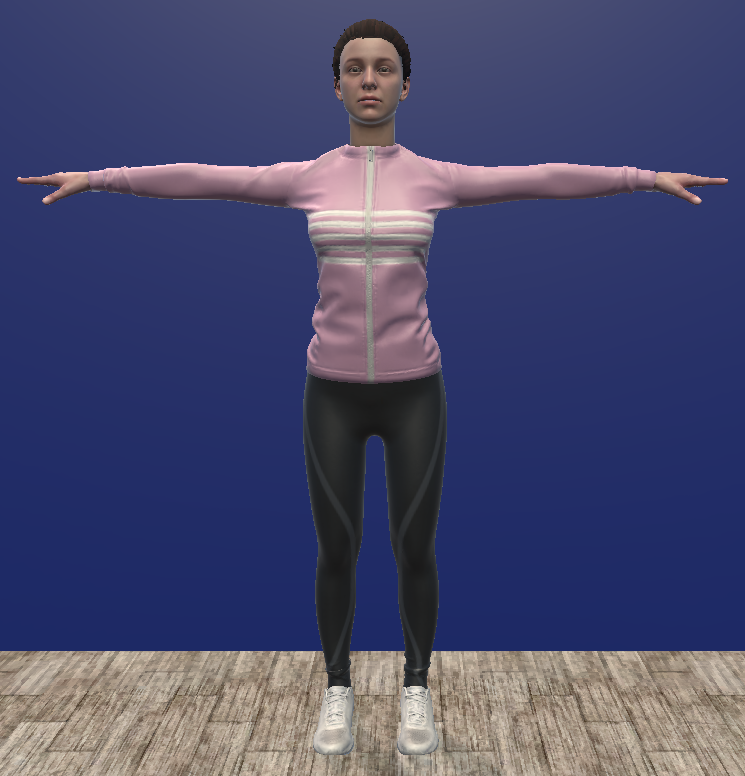
\includegraphics[width=\textwidth]{figures/Jade/Jade_Default.png}
    \caption{Jade (Mixamo) — photorealistic baseline used for initial NPR technique development.}
    \label{fig:jade_default}
  \end{subfigure}
  \hfill
  \begin{subfigure}[b]{0.45\textwidth}
    \centering
    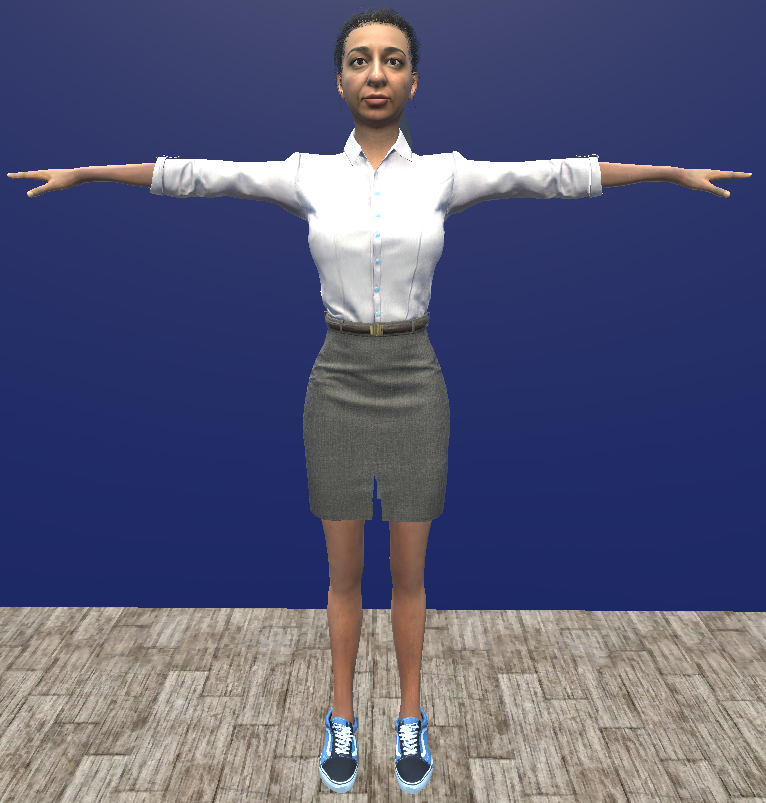
\includegraphics[width=\textwidth]{figures/Avaturn/avaturn_Default.png}
    \caption{Avaturn avatar — AI-reconstructed from a photograph, used as the primary platform for the user study.}
    \label{fig:avaturn_default}
  \end{subfigure}
  \caption{Default appearances of the two primary avatar platforms used in this thesis.}
  \label{fig:avatar_platforms}
\end{figure}

\section{NPR Technique Design}
\label{sec:technique_design}

The NPR stylisation techniques were developed through an iterative process in which each technique responds to a specific observed limitation of its predecessor. Development began on the Mixamo platform, where shader access is unrestricted, then continued within the Meta SDK environment where hook constraints shaped several implementation decisions, and was finally validated on Avaturn. What follows is a conceptual overview of each technique's motivation and visual behaviour across the three platforms. Full implementation details are provided in~\Cref{ch:implementation}.

\subsection{Shared Rendering Structure}
\label{sec:shared_structure}

All techniques share a common two-pass rendering structure. The first pass is a dedicated silhouette outline pass; the second is the main forward-lit pass in which the technique-specific NPR surface effect is computed.

The silhouette outline is generated using the inverted hull method~\cite{lake2000, isenberg2003}. Front-face culling is enabled so that only back-facing geometry is rasterised. Every vertex is displaced outward along its world-space surface normal by a configurable distance, producing an enlarged shell around the avatar. When the main pass subsequently draws the front-facing surface over the interior, the shell remains visible only at the silhouette, appearing as a solid border of controllable thickness. The displacement is performed entirely in the vertex shader, requiring no mesh preprocessing. A depth bias prevents z-fighting where the expanded shell intersects the original geometry at similar depth values.

A consistent challenge across all passes is handling semitransparent avatar geometry. Hair is typically represented as a set of flat cards with an alpha-masked texture: each card is a rectangular polygon, and the hair shape is defined by discarding fragments whose alpha value falls below a threshold. Eyelashes and eyebrow geometry use the same cutout approach. Without correct alpha handling in the outline pass, the expanded hull would be drawn across the full rectangular extent of each hair card, producing a solid rectangular border instead of a border that follows the hair silhouette. Both the outline pass and the main forward-lit pass therefore sample the base colour texture alpha channel and discard fragments below the cutout threshold before any shading or displacement is applied. This ensures that outline thickness and surface effects are consistent between the opaque body geometry and the alpha-masked regions, and that transparent areas such as the interior of the eye cornea are handled correctly.

\subsection{V1 — Toon Shading}
\label{sec:v1}

The first technique establishes the toon shading baseline. The shared silhouette outline pass provides the outer border; the forward-lit pass replaces the standard Lambertian shading with a quantized diffuse model that produces the flat, banded appearance of cartoon rendering.

The toon shading model replaces the continuous Lambertian diffuse term with a stepped function~\cite{gooch1998}. The dot product of the light direction and surface normal is divided into a configurable number of discrete bands. Each individual band boundary receives an independent smoothstep transition of controllable width, so that normal jitter near a boundary causes a narrow localised blend rather than snapping the entire surface patch between steps — a more temporally stable approach than applying a single global threshold. A Fresnel rim lighting term, approximated using Schlick's formulation~\cite{schlick1994}, brightens surface regions facing perpendicular to the viewer. A constant ambient term prevents fully shadowed regions from collapsing to black.

The Meta SDK platform implementation follows a different architectural path from the Mixamo and Avaturn variants. Rather than operating on a raw diffuse dot product, it receives the fully composited PBR output of the SDK renderer — including subsurface scattering, anisotropic hair shading, eye glints, and image-based lighting — and posterises the RGB result directly. The cel-shaded colour therefore retains the physical material quality of the underlying renderer; the stylisation abstracts its tonal range without discarding the lighting information already encoded in it.

The limitation of V1 is that the outer silhouette remains the only visible boundary. Internal surface features — facial features, clothing seams, surface creases — produce no edge signal.

\begin{figure}[H]
  \centering
  \missingfigure[figwidth=\textwidth]{V1 (Toon Shading + Geometry Outline): Mixamo (left) / Meta SDK (centre) / Avaturn (right)}
  \caption{V1 (Toon Shading with Geometry-Based Outlines) across the three avatar platforms.}
  \label{fig:v1_platforms}
\end{figure}

\subsection{V2 — X-Toon Extended Toon Shading}
\label{sec:v2}

The second technique extends the toon shading model of V1 using the X-Toon approach proposed by Barla et al.~\cite{barla2006}. Standard toon shading indexes a one-dimensional ramp texture using the Lambertian dot product between the surface normal and the light direction, which determines the diffuse shading band. X-Toon replaces this with a two-dimensional ramp texture, introducing a second lookup axis that encodes an additional scene property. In this implementation the second axis encodes the fragment's distance from the camera, allowing the shading response to vary with depth. Regions close to the viewer receive a standard toon diffuse treatment; at greater distances the ramp shifts the shading response, producing a depth-dependent variation in tone that increases perceived depth and separation between overlapping body parts.

The key advantage over V1 is expressive control over how depth reads in the final image: the designer can tune the 2D ramp texture to lighten or darken distant regions, emphasise contour separation at a chosen distance, or introduce atmospheric depth without any additional geometry. The limitation is that neither the toon model nor the 2D ramp produces any signal for interior surface detail such as facial features or clothing seams. The only visible boundary remains the outer silhouette from the shared hull pass.

\begin{figure}[H]
  \centering
  \missingfigure[figwidth=\textwidth]{V2 (X-Toon Extended Toon Shading): Mixamo (left) / Meta SDK (centre) / Avaturn (right)}
  \caption{V2 (X-Toon Extended Toon Shading) across the three avatar platforms.}
  \label{fig:v2_platforms}
\end{figure}

\subsection{V3 — Screen-Space Normal Edge Detection}
\label{sec:v3}

The third technique introduces the first interior edge signal by detecting discontinuities in the interpolated surface normal across adjacent screen pixels. The GPU hardware intrinsics \texttt{ddx} and \texttt{ddy} expose the finite difference of any fragment-stage value across a two-by-two pixel quad at negligible cost, requiring no additional texture samples. Applying this to the world-space surface normal gives a gradient magnitude as defined in~\Cref{sec:background_normal_deriv}, which responds to creases, mesh boundaries, and regions of high curvature — features that are invisible to the toon shading approaches of V1 and V2. The computation adds no texture samples to the fragment shader and executes at near-zero additional cost relative to the surrounding lighting evaluation. The key limitation is that edge thickness is measured in screen pixels and therefore scales with camera distance, producing edges that grow thinner as the avatar recedes from the viewer.

\begin{figure}[H]
  \centering
  \missingfigure[figwidth=\textwidth]{V3 (Normal Edge Detection): Mixamo (left) / Meta SDK (centre) / Avaturn (right)}
  \caption{V3 (Screen-Space Normal Edge Detection) across the three avatar platforms.}
  \label{fig:v3_platforms}
\end{figure}

\subsection{V4 — Sobel Edge Detection}
\label{sec:v4}

The fourth technique applies the Sobel operator to the avatar's diffuse albedo texture to extract colour boundaries. This captures clothing patterns, facial contour transitions, and other surface details that have no geometric counterpart. Two artefact types arise. First, UV seam boundaries produce spurious high-gradient spikes where the texture wraps discontinuously across a seam. Second, uniform skin regions produce over-detection at low thresholds because the subtle colour variation in skin tones registers as a weak but persistent edge signal. The first artefact is suppressed by a luminance range check that rejects detections where the spread of neighbourhood luminance values exceeds a configurable limit. The second is addressed by a skin classification computed per pixel based on HSV saturation that applies a stricter detection threshold in regions of low saturation.

\begin{figure}[H]
  \centering
  \missingfigure[figwidth=\textwidth]{V4 (Sobel Edge Detection): Mixamo (left) / Meta SDK (centre) / Avaturn (right)}
  \caption{V4 (Sobel Edge Detection with adaptive skin thresholding) across the three avatar platforms.}
  \label{fig:v4_platforms}
\end{figure}

\subsection{V5 — Gaussian Prefiltered Sobel}
\label{sec:v5}

The fifth technique addresses edge noise by approximating Gaussian pre-filtering before gradient computation. Following the observation of Marr and Hildreth~\cite{marr1980} that stable edge detection requires prior low-pass smoothing, this version samples the diffuse texture at a grid of offset positions and computes a weighted average before applying the Sobel operator. The smoothing reduces noise and suppresses fine texture artefacts, producing cleaner edge lines. The trade-off is a substantially higher per-fragment sample count. A further limitation is that the smoothing is spatially uniform: it softens genuine structural boundaries alongside artefacts, producing edges that are smoother in aggregate but not more selective in what they mark.

\begin{figure}[H]
  \centering
  \missingfigure[figwidth=\textwidth]{V5 (Gaussian Sobel): Mixamo (left) / Meta SDK (centre) / Avaturn (right)}
  \caption{V5 (Gaussian Prefiltered Sobel) across the three avatar platforms.}
  \label{fig:v5_platforms}
\end{figure}

\subsection{V6 — Hierarchical Edge Detection with Multiple Cues}
\label{sec:v6}

The sixth technique fuses three independent edge cues through weighted combination, addressing the limitation that no single cue reliably captures all visually meaningful boundaries. A depth proximity layer uses derivatives in screen space of the camera-to-fragment distance to detect silhouette-level boundaries. A normal layer detects surface crease edges from normal discontinuities. A colour layer applies the Roberts Cross operator to the diffuse texture to capture painted detail boundaries. The three layers are blended using weights per layer that can be adjusted at runtime, allowing the visual balance between silhouette, crease, and texture edges to be controlled interactively. This technique detects the broadest range of edge types of any approach developed to this point.

\begin{figure}[H]
  \centering
  \missingfigure[figwidth=\textwidth]{V6 (Hierarchical Multi-Cue): Mixamo (left) / Meta SDK (centre) / Avaturn (right)}
  \caption{V6 (Hierarchical Edge Detection with Multiple Cues) across the three avatar platforms.}
  \label{fig:v6_platforms}
\end{figure}

\subsection{V7 — Kuwahara Painterly Filter}
\label{sec:v7}

Rather than drawing explicit edge lines, the seventh technique applies the isotropic Kuwahara filter to the rendered surface colour to produce a painterly abstraction. For each fragment, four overlapping quadrant regions are sampled; the output is set to the mean colour of whichever quadrant has the lowest local variance. Uniform surface regions are smoothed toward a flat painterly fill, while region boundaries are sharpened implicitly because the selected quadrant is always the one that falls cleanly on one side of the boundary. This is the only technique in this thesis that does not produce explicit ink lines; the abstraction operates entirely through regional colour smoothing.

\begin{figure}[H]
  \centering
  \missingfigure[figwidth=\textwidth]{V7 (Kuwahara): Mixamo (left) / Meta SDK (centre) / Avaturn (right)}
  \caption{V7 (Kuwahara Painterly Filter) across the three avatar platforms.}
  \label{fig:v7_platforms}
\end{figure}

\subsection{V8 — Kuwahara with Sobel Edges}
\label{sec:v8}

The eighth technique combines the painterly region abstraction of V7 with the ink-line edges of V4. The Kuwahara pass is applied first to produce smooth filled regions, and Sobel edges are composited on top to add explicit contour lines. The result is a comic-book aesthetic: flat coloured regions separated by drawn boundaries. Because the edge detection runs on the abstracted Kuwahara output rather than the original diffuse texture, the lines reflect the abstracted region structure rather than every fine texture variation.

\begin{figure}[H]
  \centering
  \missingfigure[figwidth=\textwidth]{V8 (Kuwahara + Sobel): Mixamo (left) / Meta SDK (centre) / Avaturn (right)}
  \caption{V8 (Kuwahara with Sobel Edges) across the three avatar platforms.}
  \label{fig:v8_platforms}
\end{figure}

\subsection{V9 — Composite: Kuwahara, Gaussian Sobel, and Hierarchical}
\label{sec:v9}

The ninth technique chains all three main abstraction strategies into a single pipeline. The Kuwahara filter is applied first to produce the painterly base. Gaussian prefiltered Sobel edges are then composited to add smoothed colour boundary lines. Finally, the hierarchical multi-cue layer contributes depth, normal, and colour edges with independent weighting. This produces the richest visual output of any technique in the set, combining surface abstraction with two complementary edge detection strategies at the cost of the highest sample count per fragment of all techniques developed so far.

\begin{figure}[H]
  \centering
  \missingfigure[figwidth=\textwidth]{V9 (Composite): Mixamo (left) / Meta SDK (centre) / Avaturn (right)}
  \caption{V9 (Composite: Kuwahara, Gaussian Sobel, Hierarchical) across the three avatar platforms.}
  \label{fig:v9_platforms}
\end{figure}

\section{Technique Selection for the User Study}
\label{sec:technique_selection}

Following the iterative development phase, a single technique is selected for the NPR condition in the user study based on visual assessment across all three avatar platforms. Three criteria guide the selection. First, facial expression detail must remain readable under the stylisation, since the study measures trust responses to a speaking avatar. Second, the effect must be visually coherent across viewing distances, since the video scenarios are filmed at a fixed conversational distance. Third, the abstraction must be clearly distinct from the photorealistic baseline to ensure that any difference in trust ratings reflects a genuine perceptual response to the stylisation. The outcome of this assessment is documented in~\Cref{ch:evaluation}.

\section{User Study Design}
\label{sec:user_study}

\subsection{Objective and Hypotheses}
\label{sec:study_objective}

The user study addresses RQ3 by measuring how the visual representation of a speaker affects the perceived trustworthiness of their advice in a concrete decision situation. Three presentation conditions are compared: a real human speaker, a photorealistic Avaturn avatar, and an Avaturn avatar rendered with NPR stylisation. Two hypotheses are tested.

\textbf{H1:} Participants will rate the real-person condition as most trustworthy, establishing a human baseline against which avatar conditions can be compared.

\textbf{H2:} The NPR-stylised avatar will not be rated significantly less trustworthy than the photorealistic avatar, and may be rated more trustworthy if the photorealistic condition triggers uncanny valley discomfort.

\subsection{Conditions}
\label{sec:study_conditions}

The study compares three presentation conditions:

\begin{description}
  \item[C0 — Real Person:] A video recording of a real human speaker delivering the recommendation. This serves as the trust ceiling baseline.
  \item[C1 — Photorealistic Avatar:] The same speaker scenario rendered using a photorealistic Avaturn avatar with standard PBR shading. Facial expressions are driven by blendshape animation to match the delivery timing.
  \item[C2 — NPR Avatar:] The Avaturn avatar rendered with the NPR technique selected from the visual assessment as providing the best balance of abstraction and expressiveness.
\end{description}

\subsection{Scenarios}
\label{sec:study_scenarios}

Three video scenarios are designed to present naturalistic decisions in which the speaker's trustworthiness is relevant. Each scenario introduces a situation with two plausible options and shows the speaker recommending one. The scenarios are kept domain-neutral to avoid prior knowledge effects. After watching each video, participants rate how trustworthy they found the speaker's recommendation.

Scenario content, option framing, and speaker delivery are held constant across conditions; only the visual presentation of the speaker changes. The three scenarios are counterbalanced across conditions using a Latin square to control for scenario-condition order effects.

\subsection{Procedure and Measures}
\label{sec:study_procedure}

The study uses a within-subjects design. Each participant watches all three conditions across the three scenarios, with condition-scenario assignment randomised per participant. After each video, participants complete a short questionnaire including a trust rating scale and items from the Godspeed questionnaire~\cite{macdorman2006} assessing human-likeness and eeriness.

Within-subjects differences across the three conditions are analysed using a repeated-measures design. Pairwise comparisons between each avatar condition and the real-person baseline, and between the two avatar conditions, are conducted with Bonferroni correction. Effect sizes are reported as partial $\eta^2$.

\subsection{Ethical Considerations}
\label{sec:study_ethics}

The study was reviewed and approved by the University of Konstanz ethics committee. Participants provided written informed consent before participation. Data is anonymised at collection; no personally identifiable information is stored alongside questionnaire responses. Participation was voluntary with the right to withdraw at any time.

%% Chapter 5 — Implementation
\chapter{Implementation}
\label{ch:implementation}

This chapter documents the technical realisation of the NPR avatar system. It covers the development environment, the integration path for each avatar platform, the implementation of the shared rendering structure, and the HLSL-level details of each stylisation technique developed to date. Runtime tooling developed to support iterative development is described at the end of the chapter.

\section{Development Environment}
\label{sec:impl_environment}

The system was developed in Unity~6 (version 6000.0.60f1) using the Universal Render Pipeline~(URP). The target hardware is the Meta Quest family of standalone VR headsets. The Meta Avatars SDK version~40.0.1 was used for the SDK-managed avatar platform. All shader code is written in HLSL and targets the URP forward rendering path.

\section{Avatar Platform Integration}
\label{sec:impl_platforms}

\subsection{Mixamo}
\label{sec:impl_mixamo}

Mixamo characters are exported as FBX assets and imported into Unity as standard skinned mesh renderers. No proprietary shader system is involved, so all URP materials can be replaced directly with custom NPR shaders without restriction. The Mixamo character Jody served as the primary prototyping target during technique development, allowing the NPR shaders to be iterated freely before the more constrained platform integrations were addressed.

\subsection{Meta Avatars SDK}
\label{sec:impl_meta}

The Meta Avatars SDK manages avatar materials through its Extensible Shader Framework~(ESF), which generates platform-specific HLSL from parameterised templates. The generated source is not intended to be edited directly. Custom logic is instead injected through named hook functions that the ESF exposes at defined points in the shader pipeline.

The hook used in this thesis is \texttt{AppSpecificPostManipulation}, which executes per fragment after all SDK PBR lighting — subsurface scattering, eye glints, hair shading — has been computed. It receives the accumulated lit colour and returns a modified colour, giving full control over the final fragment output without disrupting any SDK rendering logic. The hook is defined across three files that the ESF includes automatically during shader compilation:

\begin{itemize}
  \item \texttt{app\_functions.hlsl} — the body of \texttt{AppSpecificPostManipulation}; dispatches to the active NPR technique based on the \texttt{\_NPREffect} keyword
  \item \texttt{app\_declarations.hlsl} — uniform declarations for all NPR parameters, shared across techniques
  \item \texttt{app\_variants.hlsl} — shader feature keyword declarations that activate each technique branch
\end{itemize}

A further complication is the SDK's LOD management system, which replaces avatar materials automatically as camera distance changes. This reverts any custom shader assignment made at load time. The \texttt{AvatarShaderSwapper.cs} script addresses this by running a periodic coroutine that re-applies the custom NPR materials after each LOD transition is detected. The script also handles the initial material replacement, waiting for the asynchronous avatar load to complete before copying base colour and normal textures from the SDK materials into the custom shader properties.

\subsection{Avaturn}
\label{sec:impl_avaturn}

Avaturn exports avatars in the \texttt{.glb} format, the binary container of the glTF~2.0 standard. Unity does not natively support runtime glTF loading, so the GLTFast package is used to load the asset at runtime. On load completion, GLTFast produces a standard Unity GameObject hierarchy with skinned mesh renderers and PBR materials assigned from the glTF material definitions, including albedo, normal, and metallic-roughness textures. Because Avaturn avatars carry no proprietary shader constraints once imported, the custom NPR materials are assigned to the resulting skinned meshes using the same approach as Mixamo: direct material replacement after load. Blendshape animation targets exported by Avaturn are preserved through the GLTFast import and driven at runtime via \texttt{SkinnedMeshRenderer.SetBlendShapeWeight} for the video recording scenarios used in the user study.

\section{Shared Rendering Structure}
\label{sec:impl_shared}

The NPR shader used across Mixamo and Avaturn is \texttt{Avatar-Meta-UGB.shader}, a multi-pass URP shader containing two passes: \texttt{NPROutline} and \texttt{ForwardLit}. For the Meta SDK platform, the forward-lit NPR logic runs inside \texttt{AppSpecificPostManipulation}; the outline pass is handled by a separate material applied to a duplicate mesh layer.

The core forward-lit dispatch lives in \texttt{Style2MetaAvatarCore.hlsl}. It reads the active \texttt{\_NPREffect} shader keyword and branches to the corresponding technique include file. This structure means all eight techniques share the same entry point and parameter infrastructure; switching techniques at runtime requires only toggling the active keyword via \texttt{Material.EnableKeyword} and \texttt{Material.DisableKeyword}, which the runtime UI performs without recompilation.

\subsection{Inverted Hull Outline Pass}
\label{sec:impl_outline}

The outline pass implements the inverted hull silhouette. In the Mixamo and Avaturn shaders the pass sets \texttt{Cull Front}, \texttt{ZWrite On}, \texttt{ZTest Less}; in the Meta SDK shader it sets \texttt{Cull Front}, \texttt{ZWrite Off}, \texttt{ZTest LEqual} to avoid conflicting with the SDK's depth compositing. The vertex shader displaces each vertex outward along its world-space normal by \texttt{\_OuterOutlineWidth} (Mixamo/Avaturn, world-space metres) or \texttt{\_OutlineWidth * 0.001} (Meta, converted from UI units). The fragment outputs a flat \texttt{\_OuterOutlineColor} or \texttt{\_OutlineColor}. An \texttt{\_OutlineDepthBias} property shifts the clip-space Z coordinate toward the camera to prevent z-fighting where the expanded shell and the original surface meet at shallow angles.

\subsection{Alpha Cutout Handling}
\label{sec:impl_alpha}

Alpha cutout is controlled by the \texttt{\_EnableAlphaTest} flag rather than being always-on. When enabled, both the outline pass and the forward-lit pass sample the base colour texture alpha channel and call \texttt{clip(alpha - threshold)} before any displacement or shading is applied. In the outline pass this ensures the expanded hull is discarded wherever the hair card texture is transparent, preventing a rectangular border from appearing around each card. The cutout threshold is exposed in the runtime UI and adjusted per avatar submesh — a lower threshold is typically used for eyelashes (dense geometry) than for hair cards (sparse, large transparent regions).

\section{NPR Technique Implementation}
\label{sec:impl_techniques}

\subsection{V1 — Toon Shading}
\label{sec:impl_v1}

Three separate shader implementations exist for V1, one per avatar platform. The outline pass is structurally identical across all three (inverted hull, normal-offset displacement, alpha cutout); the toon shading pass differs because the Mixamo and Avaturn variants operate on raw NdotL, while the Meta variant operates on the composited PBR output.

\subsubsection{Mixamo}
\label{sec:impl_v1_mixamo}

\textbf{Shader:} \texttt{Assets/AvatarShaderExperimental/Shaders/V1\_ToonShading\_GeometryOutline.shader} \\
\textbf{Pipeline target:} URP, \texttt{\#pragma target 3.0}

The outline pass sets \texttt{Cull Front}, \texttt{ZWrite On}, \texttt{ZTest Less} and displaces each vertex along its world-space normal by \texttt{\_OuterOutlineWidth} (world units). The fragment returns a flat \texttt{\_OuterOutlineColor}. When \texttt{\_EnableAlphaTest} is active, a \texttt{clip} call discards fragments below the alpha threshold before any displacement is applied, ensuring the hull respects hair card silhouettes. An \texttt{\_OutlineDepthBias} value shifts clip-space Z toward the camera to prevent z-fighting at shallow angles.

The toon pass quantises the Lambertian dot product $\mathbf{N} \cdot \mathbf{L}$ per step using a per-band smoothstep. The expression after unification with the Avaturn version is:

\begin{lstlisting}[language=C, style=mystyle, caption={V1 toon quantisation — Mixamo and Avaturn (unified).}]
float steps  = max(1.0, _ToonSteps);
float scaled = NdotL * steps;
float band   = floor(scaled);
float frac   = scaled - band;
float blend  = smoothstep(1.0 - _ToonSmoothness, 1.0, frac);
float toon   = saturate((band + blend) / steps);
toon = lerp(1.0 - _ShadowStrength, 1.0, toon);
\end{lstlisting}

Each band boundary receives an independent narrow blend of width \texttt{\_ToonSmoothness}, so normal jitter near any seam produces a localised crossfade rather than snapping the whole surface patch between bands. Vertex positions and normals are read directly from the standard mesh attributes; no compute-skinning bridge is needed for standard \texttt{Skinned\-Mesh\-Renderer} avatars. An additive ambient \texttt{\_AmbientColor} and a rim term \texttt{pow(1 - NdotV, RimPower)} are added to the quantised diffuse.

\subsubsection{Avaturn}
\label{sec:impl_v1_avaturn}

\textbf{Shader:} \texttt{Assets/Shaders/NPR/V1\_ToonShading\_GeometryOutline.shader} \\
\textbf{Pipeline target:} URP, \texttt{\#pragma target 3.5} \\
\textbf{Materials:} five materials covering body, head, hair, eyelash, and look submeshes

The toon pass uses the same per-step quantisation as Mixamo (Listing~5.1). The outline pass is structurally identical to Mixamo with one critical addition: before computing world positions, the vertex shader calls \texttt{OVR\_FETCH\_POS\_NORM(v.vertex.xyz, v.normal, v.vertexID)}. This bridge reads vertex positions and normals from the external compute-skinned vertex buffers written by the Meta SDK runtime. Without it, the GPU-skinned vertices are not visible to the vertex shader, and the outline hull renders at the bind-pose position. The same bridge is required in the toon pass for correct deformation tracking. For standard Avaturn avatars loaded via GLTFast without the Meta SDK runtime, the macro resolves to a no-op and the attributes fall back to the standard mesh inputs.

\subsubsection{Meta Avatars SDK}
\label{sec:impl_v1_meta}

\textbf{Shader:} \texttt{Assets/Shaders/CustomShaders/Avatar-Meta-UGB.shader} \\
\textbf{Keyword:} \texttt{EFFECT\_TOON} (enabled via \texttt{ENABLE\_NPR\_EDGES}) \\
\textbf{Technique file:} \texttt{Assets/Shaders/CustomShaders/NPREffect\_Toon.cginc}

The Meta implementation runs inside \texttt{AppSpecificPostManipulation}, which receives the fully composited PBR colour produced by the SDK's \texttt{STYLE\_2\_STANDARD} renderer. The quantisation therefore operates on RGB directly, preserving hue while stepping luminance:

\begin{lstlisting}[language=C, style=mystyle, caption={V1 posterisation — Meta SDK (\texttt{NPREffect\_Toon.cginc}).}]
float  bands      = max(2.0, _ToonColorBands);
float3 posterized = floor(color.rgb * bands + 0.5) / bands;
color.rgb = lerp(color.rgb, posterized, _ToonPosterizeStrength);

float lum  = dot(color.rgb, float3(0.2126, 0.7152, 0.0722));
color.rgb  = lerp(float3(lum, lum, lum), color.rgb, _ToonSaturation);
\end{lstlisting}

The \texttt{floor(rgb * bands + 0.5) / bands} expression rounds each channel to the nearest multiple of $1/\text{bands}$ (round-to-nearest rather than floor-to-band), which distributes quantisation error symmetrically and avoids the darkening bias of a plain floor. Saturation adjustment runs after posterisation to prevent clamping artefacts. Because the input already contains Meta's subsurface scattering, anisotropic hair, and eye glints, the posterised output stylises a physically correct image rather than reconstructing lighting from scratch.

The outline pass in this shader is a dedicated \texttt{NPROutline} pass with \texttt{Cull Front}, \texttt{ZWrite Off}, \texttt{ZTest LEqual}. The vertex shader displaces each SDK-skinned vertex outward by:

\begin{lstlisting}[language=C, style=mystyle, caption={Outline vertex displacement — Meta SDK outline pass.}]
float3 worldPos = o.v_WorldPos + normalize(o.v_Normal) * _OutlineWidth * 0.001;
\end{lstlisting}

The \texttt{0.001} scale converts \texttt{\_OutlineWidth} from millimetre-scale UI units to metre-scale world space. The outline is toggled via \texttt{\_OutlineEnabled}; the fragment discards if the value is below 0.5. Unlike the Mixamo and Avaturn variants, \texttt{ZWrite Off} is used because the Meta pipeline already has correct depth from the main pass and a second depth write would cause artefacts with the SDK's transparency compositing.

\begin{table}[H]
  \centering
  \caption{V1 implementation comparison across the three avatar platforms.}
  \label{tab:v1_comparison}
  \small
  \begin{tabularx}{\textwidth}{lXXX}
    \toprule
    & \textbf{Mixamo} & \textbf{Avaturn} & \textbf{Meta SDK} \\
    \midrule
    Quantisation method & Per-step smoothstep, NdotL & Per-step smoothstep, NdotL & Round-to-nearest, composited RGB \\
    Skinning bridge & None & \texttt{OVR\_FETCH\_POS\_NORM} & SDK native \\
    Rim light & Additive, computed & Additive, computed & Pre-composited by Meta PBR \\
    Outline depth write & \texttt{ZWrite On} & \texttt{ZWrite On} & \texttt{ZWrite Off} \\
    Outline toggleable & No & No & Yes (\texttt{\_OutlineEnabled}) \\
    Shadow source & URP \texttt{GetMainLight} & URP cascades & Meta PBR attenuation \\
    \bottomrule
  \end{tabularx}
\end{table}

\begin{figure}[H]
  \centering
  \missingfigure[figwidth=\textwidth]{V1 (Toon Shading): Mixamo (left) / Meta SDK (centre) / Avaturn (right)}
  \caption{V1 (Toon Shading) across the three avatar platforms.}
  \label{fig:v1_impl}
\end{figure}

\subsection{V2 — X-Toon Extended Toon Shading}
\label{sec:impl_v2}

The X-Toon implementation replaces the procedural quantization of V1 with a lookup into a two-dimensional ramp texture, \texttt{\_ToonRampTex}. The horizontal axis of the ramp is indexed by the Lambertian dot product $\mathbf{N} \cdot \mathbf{L}$, remapped from $[-1, 1]$ to $[0, 1]$. The vertical axis is indexed by a depth factor derived from the linear eye-space depth of the fragment, normalised against a configurable \texttt{\_DepthRange} parameter. Sampling the ramp with these two coordinates produces a colour that encodes both the diffuse shading band and its depth-dependent modification. The Fresnel rim and ambient terms from V1 are retained. The ramp texture itself is authored externally and assigned as a material property, giving the designer full control over the shading character without shader recompilation.

\begin{figure}[H]
  \centering
  \missingfigure[figwidth=\textwidth]{V2 (X-Toon): Mixamo (left) / Meta SDK (centre) / Avaturn (right)}
  \caption{V2 (X-Toon Extended Toon Shading) across the three avatar platforms.}
  \label{fig:v2_impl}
\end{figure}

\subsection{V3 — Screen-Space Normal Edge Detection}
\label{sec:impl_v3}

The normal edge implementation uses the \texttt{ddx} and \texttt{ddy} hardware intrinsics applied to the interpolated world-space surface normal $\mathbf{N}$, which is available as a fragment-stage interpolant at no additional texture sample cost. The gradient magnitude is computed as $M_N = \sqrt{\|\texttt{ddx}(\mathbf{N})\|^2 + \|\texttt{ddy}(\mathbf{N})\|^2}$, producing a scalar per fragment that is high at surface creases, mesh boundaries, and regions of high curvature. This value is compared against \texttt{\_NormalThreshold}; fragments exceeding the threshold are output as \texttt{\_EdgeColor}, and all others pass the base albedo through unchanged. An optional \texttt{\_NormalEdgePower} exponent controls the response curve, allowing soft crease edges to be suppressed relative to sharp geometric boundaries.

\begin{figure}[H]
  \centering
  \missingfigure[figwidth=\textwidth]{V3 (Normal Edge Detection): Mixamo (left) / Meta SDK (centre) / Avaturn (right)}
  \caption{V3 (Screen-Space Normal Edge Detection) across the three avatar platforms.}
  \label{fig:v3_impl}
\end{figure}

\subsection{V4 — Sobel Edge Detection}
\label{sec:impl_v4}

The Sobel implementation samples the diffuse albedo texture at eight neighbours in a $3\times3$ grid centred on the current fragment, using a fixed texel offset \texttt{\_TexelSize}. The horizontal and vertical gradient components $G_x$ and $G_y$ are accumulated using the Sobel kernel weights, and the edge magnitude is computed as $M = \sqrt{G_x^2 + G_y^2}$.

Two artefact suppression mechanisms are applied before the threshold test. The luminance range check computes the spread of luminance values across the nine samples; if the spread exceeds \texttt{\_SeamRangeLimit}, the pixel is rejected as a UV seam artefact. The skin classification converts the centre sample to HSV and compares the saturation channel against \texttt{\_SkinSaturationCutoff}; fragments below the cutoff are classified as skin and tested against a stricter threshold \texttt{\_SkinEdgeThreshold} rather than the standard \texttt{\_EdgeThreshold}. Fragments exceeding the active threshold are coloured \texttt{\_EdgeColor}; all others pass through the base albedo.

\begin{figure}[H]
  \centering
  \missingfigure[figwidth=\textwidth]{V4 (Sobel): Mixamo (left) / Meta SDK (centre) / Avaturn (right)}
  \caption{V4 (Sobel Edge Detection) across the three avatar platforms.}
  \label{fig:v4_impl}
\end{figure}

\subsection{V5 — Gaussian Prefiltered Sobel}
\label{sec:impl_v5}

The Gaussian prefiltered Sobel implementation adds a smoothing stage before gradient computation. A $5\times5$ sample grid is evaluated at the current fragment, with each sample weighted by a precomputed Gaussian coefficient derived from a standard deviation \texttt{\_GaussianSigma}. The weighted sum produces a smoothed colour estimate at each of the nine Sobel positions. The Sobel gradient is then applied to the smoothed values rather than the raw texture samples. Because the Gaussian and Sobel stages both require neighbourhood samples, the total sample count for this technique is higher than V4; the exact count depends on the kernel radius configured via \texttt{\_GaussRadius}. The artefact suppression mechanisms from V4 are retained.

\begin{figure}[H]
  \centering
  \missingfigure[figwidth=\textwidth]{V5 (Gaussian Sobel): Mixamo (left) / Meta SDK (centre) / Avaturn (right)}
  \caption{V5 (Gaussian Prefiltered Sobel) across the three avatar platforms.}
  \label{fig:v5_impl}
\end{figure}

\subsection{V6 — Hierarchical Edge Detection}
\label{sec:impl_v6}

The hierarchical implementation computes three independent edge layers in a single fragment shader invocation and combines them via weighted addition.

The depth layer uses \texttt{ddx} and \texttt{ddy} applied to the fragment's linear eye depth to estimate the depth gradient magnitude. The gradient is normalised by \texttt{\_DepthSensitivity} and thresholded to produce a binary edge signal. The normal layer applies the same derivative approach to the interpolated world-space surface normal vector, computing $M_N = \sqrt{\|\texttt{ddx}(\mathbf{N})\|^2 + \|\texttt{ddy}(\mathbf{N})\|^2}$ and thresholding against \texttt{\_NormalThreshold}. The colour layer applies the Roberts Cross operator to the diffuse texture: it samples four neighbours in a $2\times2$ diagonal pattern and computes the cross-difference magnitudes $|R_1|$ and $|R_2|$ as defined in~\Cref{sec:background_gradient}, thresholded against \texttt{\_ColorThreshold}.

The three binary edge signals are weighted by \texttt{\_DepthWeight}, \texttt{\_NormalWeight}, and \texttt{\_ColorWeight} respectively and summed. The combined weight is clamped to $[0,1]$ and used to blend between the base albedo and \texttt{\_EdgeColor}.

\begin{figure}[H]
  \centering
  \missingfigure[figwidth=\textwidth]{V6 (Hierarchical): Mixamo (left) / Meta SDK (centre) / Avaturn (right)}
  \caption{V6 (Hierarchical Edge Detection) across the three avatar platforms.}
  \label{fig:v6_impl}
\end{figure}

\subsection{V7 — Kuwahara Painterly Filter}
\label{sec:impl_v7}

The Kuwahara implementation evaluates four overlapping quadrant subregions around the current fragment. Each quadrant is a square of radius \texttt{\_KuwaharaRadius}, offset from the centre so that adjacent quadrants share a one-texel border. For each quadrant, the implementation accumulates the sum and sum-of-squares of the sampled colour values, then computes the per-channel mean and variance from these accumulators. The quadrant with the lowest luminance variance is selected, and its mean colour is written as the fragment output.

Because the filter operates on the diffuse texture using fixed texture-coordinate offsets, no intermediate render target is required, and the entire computation runs inside the single-pass fragment hook. The isotropic formulation is used; the anisotropic extension of Kyprianidis et al.~\cite{kyprianidis2009} requires a structure tensor computed in a prior pass and is therefore incompatible with the single-pass constraint of the Meta SDK hook.

\begin{figure}[H]
  \centering
  \missingfigure[figwidth=\textwidth]{V7 (Kuwahara): Mixamo (left) / Meta SDK (centre) / Avaturn (right)}
  \caption{V7 (Kuwahara Painterly Filter) across the three avatar platforms.}
  \label{fig:v7_impl}
\end{figure}

\subsection{V8 — Kuwahara with Sobel Edges}
\label{sec:impl_v8}

The V8 implementation chains the Kuwahara and Sobel stages in sequence within the same fragment shader invocation. The Kuwahara filter is applied first, producing a smoothed mean colour from the lowest-variance quadrant. The Sobel gradient is then computed using the Kuwahara output as the input signal rather than the raw diffuse texture. Because the Kuwahara output is piecewise uniform within regions, the Sobel operator responds primarily to inter-region boundaries, suppressing the fine texture gradients that produce noise in V4. The skin saturation and seam rejection checks from V4 are retained. The detected edges are composited over the Kuwahara output using \texttt{\_EdgeColor} and \texttt{\_EdgeThreshold}.

\begin{figure}[H]
  \centering
  \missingfigure[figwidth=\textwidth]{V8 (Kuwahara + Sobel): Mixamo (left) / Meta SDK (centre) / Avaturn (right)}
  \caption{V8 (Kuwahara with Sobel Edges) across the three avatar platforms.}
  \label{fig:v8_impl}
\end{figure}

\subsection{V9 — Composite: Kuwahara, Gaussian Sobel, and Hierarchical}
\label{sec:impl_v9}

The composite technique chains three stages. First, the Kuwahara filter produces the painterly base. Second, the Gaussian prefiltered Sobel is applied to the Kuwahara output to extract smoothed colour boundary lines. Third, the hierarchical depth, normal, and Roberts Cross edge layers are evaluated and composited on top of the Gaussian Sobel result with independent weighting. All three stages share the same input texture and are computed sequentially within the single fragment shader invocation. The total sample count is the sum of the Kuwahara quadrant samples, the Gaussian prefilter samples, and the four Roberts Cross samples, making this the most sample-intensive technique developed to date.

\begin{figure}[H]
  \centering
  \missingfigure[figwidth=\textwidth]{V9 (Composite): Mixamo (left) / Meta SDK (centre) / Avaturn (right)}
  \caption{V9 (Composite: Kuwahara, Gaussian Sobel, Hierarchical) across the three avatar platforms.}
  \label{fig:v9_impl}
\end{figure}

\section{Runtime Tooling}
\label{sec:impl_tooling}

\subsection{In-VR Parameter Tuning Interface}
\label{sec:impl_ui}

\texttt{NPREdgeDetectionUI.cs} implements a fully procedural WorldSpace UI panel that is visible and interactive from inside the headset. The panel is constructed at runtime from Unity UI primitives: each tunable parameter is represented by a labelled row containing either a slider or a toggle button, laid out in technique-specific groups. Controller raycasting using the OVR interaction layer detects when the ray from either controller intersects a slider's \texttt{BoxCollider}; a trigger-pull gesture initiates a drag interaction that maps horizontal ray movement to the slider's value range. Technique switching is handled through a dropdown row: selecting a technique calls \texttt{EnableKeyword} and \texttt{DisableKeyword} on the active materials to swap the active shader branch without recompilation.

The panel exposes parameters across all technique groups, including per-technique thresholds, weights, kernel radii, and colour properties. This tool was central to the visual assessment process used to select the technique for the user study.

\subsection{LOD Material Management}
\label{sec:impl_swapper}

\texttt{AvatarShaderSwapper.cs} solves the material reversion problem described in~\Cref{sec:impl_meta}. On startup it subscribes to the avatar load completion callback and performs an initial material replacement pass across all LOD levels. A coroutine running at a configurable polling interval inspects the active materials on each renderer at runtime; if an SDK-assigned material is detected — indicating that a LOD transition has reverted the custom assignment — the coroutine re-applies the NPR material and copies the base colour and normal texture references from the newly active SDK material into the replacement shader's properties.

\subsection{Pose Freeze for Evaluation}
\label{sec:impl_freeze}

\texttt{AvatarFreezeController.cs} enables the avatar's body-tracking pose to be frozen at a chosen instant, preserving a specific expression and body posture for evaluation screenshots. The freeze is implemented by accessing the \texttt{\_inputTrackingProvider} field of \texttt{OvrAvatarInputManager} via reflection and substituting a snapshot provider that returns a fixed pose state. Pressing A, X, or the Space key toggles the freeze on and off.

%% Chapter 6 — Evaluation
\chapter{Evaluation}
\label{ch:evaluation}

This chapter evaluates the implemented NPR avatar system and documents the planned user study for trust assessment.

\section{Technical Evaluation Setup}
\label{sec:technical_setup}

\subsection{Evaluation Objectives}

The technical evaluation verifies:
\begin{itemize}
  \item the quality and coherence of NPR avatar rendering in VR
  \item real-time performance and stability under realistic usage
  \item readiness of the system for a trust-focused user study.
\end{itemize}

\subsection{Technical Metrics}

Define the quantitative and qualitative metrics:
\begin{itemize}
  \item average frame rate and minimum frame rate
  \item frame time variance and rendering latency
  \item stylization fidelity indicators such as edge coherence and temporal stability
  \item subjective observations from developer-led test sessions.
\end{itemize}

\subsection{Baseline Comparisons}

List the technical baselines used for comparison:
\begin{itemize}
  \item non-stylized VR avatar rendering
  \item existing NPR avatar rendering approaches, if available
  \item simplified style variants to isolate the effect of each component.
\end{itemize}

\section{Implementation Validation}
\label{sec:implementation_validation}

\subsection{Performance Results}

Summarize measured performance:
\begin{itemize}
  \item frame rate and latency results in representative VR scenarios
  \item resource usage on target hardware
  \item performance behavior for each style variant.
\end{itemize}

\subsection{Visual Quality Assessment}

Report qualitative observations and comparisons:
\begin{itemize}
  \item visual consistency across head motion
  \item edge quality, shading coherence, and stylization clarity
  \item artifacts or failure cases observed during testing.
\end{itemize}

\subsection{Stability and Robustness}

Describe the stability of the implementation:
\begin{itemize}
  \item behavior during extended VR sessions
  \item integration issues and debugging outcomes
  \item support for varying avatar animations and scene complexity.
\end{itemize}

\section{User Study Design}
\label{sec:user_study_design}

This section describes the planned user study that will assess how NPR avatar styles influence trust.

\subsection{Study Goals}

The study aims to answer:
\begin{itemize}
  \item how do different NPR avatar styles affect perceived trustworthiness in VR?
  \item which visual traits most strongly influence trust and social presence?
  \item does performance or visual quality moderate trust judgments?
\end{itemize}

\subsection{Participants and Recruitment}

Define the participant pool and recruitment plan:
\begin{itemize}
  \item target sample size and demographics
  \item inclusion and exclusion criteria
  \item ethical considerations and informed consent.
\end{itemize}

\subsection{Experimental Conditions}

Describe the conditions participants will experience:
\begin{itemize}
  \item baseline avatar rendering
  \item multiple NPR avatar variants with different stylization levels
  \item within-subject or between-subject study design.
\end{itemize}

\subsection{Task Scenario}

Outline the interaction scenario used in the study:
\begin{itemize}
  \item task or dialog with the avatar
  \item session duration and condition order
  \item behavioural measures such as task completion or response time.
\end{itemize}

\subsection{Measurement Instruments}

List the trust and presence instruments:
\begin{itemize}
  \item trust questionnaire adapted from VR or HRI research
  \item presence / immersion scale
  \item post-condition ratings for comfort, realism, and trust
  \item optional behavioural metrics such as interaction choices.
\end{itemize}

\subsection{Pilot Study Plan}

Describe the pilot study to validate the protocol:
\begin{itemize}
  \item a small pilot participant set
  \item testing condition order, questionnaire clarity, and timing
  \item refining instructions and VR content before the full study.
\end{itemize}

\section{Discussion}
\label{sec:discussion}

Reflect on the implementation and readiness for the user study.

\subsection{Readiness for the User Study}

Summarize whether the current system is ready for the planned study and what remains to be done.

\subsection{Limitations}

Discuss limitations affecting the planned study:
\begin{itemize}
  \item hardware and platform constraints
  \item asset and style coverage limitations
  \item potential bias in the selected stylization conditions.
\end{itemize}

%% Chapter 7 — Conclusion
\chapter{Conclusion}
\label{ch:conclusion}

\section{Summary}
\label{sec:summary}

This thesis presented \ldots. We introduced \ldots\ and demonstrated that \ldots.

The main contributions can be summarized as follows:

\begin{itemize}
  \item We proposed \ldots, which achieves \ldots.
  \item We showed that \ldots.
  \item We provided an open-source implementation and evaluation on \ldots.
\end{itemize}

\section{Limitations}
\label{sec:limitations}

Despite the promising results, the proposed approach has the following limitations:

\begin{itemize}
  \item \textbf{Limitation 1:} \ldots
  \item \textbf{Limitation 2:} \ldots
\end{itemize}

\section{Future Work}
\label{sec:future_work}

Several directions for future research are identified:

\begin{itemize}
  \item \textbf{Direction 1:} \ldots
  \item \textbf{Direction 2:} \ldots
  \item \textbf{Direction 3:} \ldots
\end{itemize}


%% ---- Back Matter ----
\backmatter
\printbibliography[heading=bibintoc]
\appendix
%% Appendix A
\chapter{Additional Results}
\label{app:additional_results}

This appendix contains supplementary results that support the findings in \Cref{ch:evaluation} but were omitted from the main body for conciseness.

\section{Extended Quantitative Comparison}
\label{app:extended_quant}

\lipsum[1]

\section{Additional Qualitative Examples}
\label{app:qual_examples}

\lipsum[2]

\section{Hyperparameter Sensitivity}
\label{app:hyperparams}

\lipsum[3]


\end{document}
